\documentclass{article}
\usepackage{graphicx}
\usepackage{geometry}
\geometry{a4paper, margin=1in}

\begin{document}

\section*{Appendix: Visual Examples}\label{sec:appendix_images}

\subsection*{Maze Map}

\subsubsection*{Manhattan}
\begin{figure}[!ht]
    \centering
    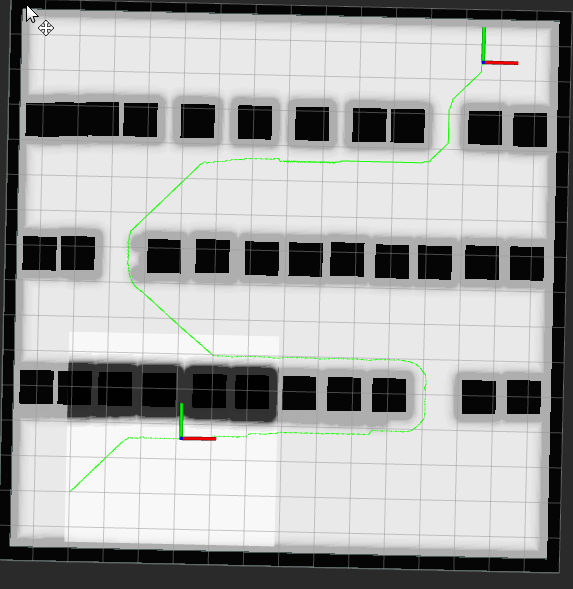
\includegraphics[width=0.9\columnwidth]{../images/manhattan_maze_corridor.png}
    \caption{Maze map: Manhattan heuristic.}
    \label{fig:manhattan_maze}
\end{figure}
\clearpage

\subsubsection*{Euclidean}
\begin{figure}[!ht]
    \centering
    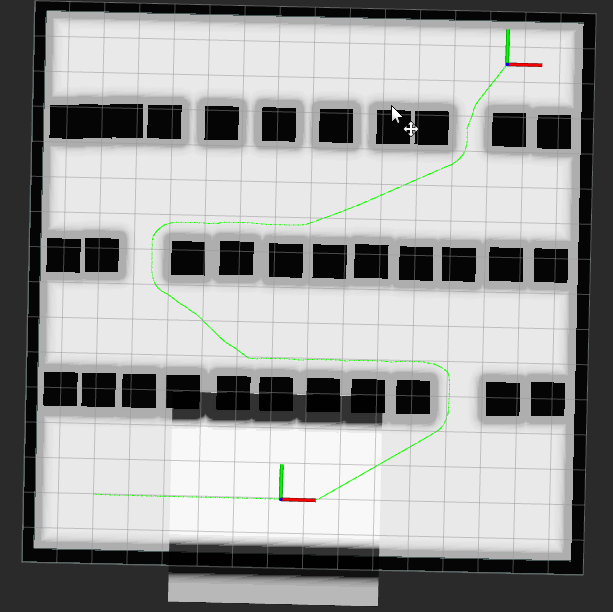
\includegraphics[width=0.9\columnwidth]{../images/euclidian_maze_corridor.png}
    \caption{Maze map: Euclidean heuristic.}
    \label{fig:euclidean_maze}
\end{figure}
\clearpage

\subsubsection*{Chebyshev}
\begin{figure}[!ht]
    \centering
    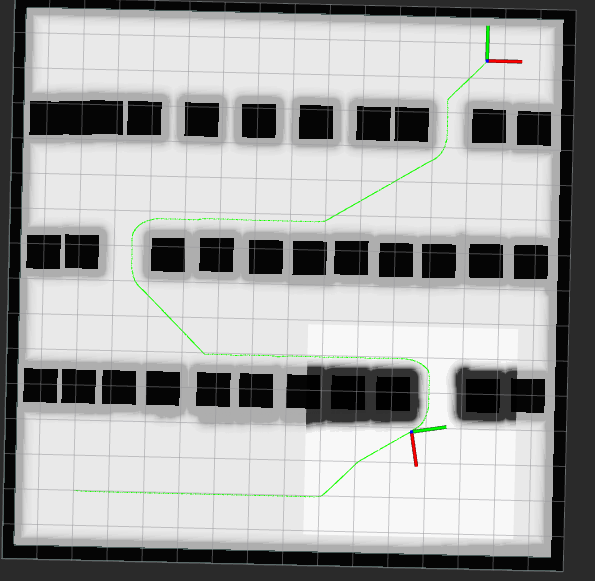
\includegraphics[width=0.9\columnwidth]{../images/chebyshecv_maze_corridor.png}
    \caption{Maze map: Chebyshev heuristic.}
    \label{fig:chebyshev_maze}
\end{figure}

\clearpage

\subsection*{Blank Map}

\subsubsection*{Manhattan}
\begin{figure}[!ht]
    \centering
    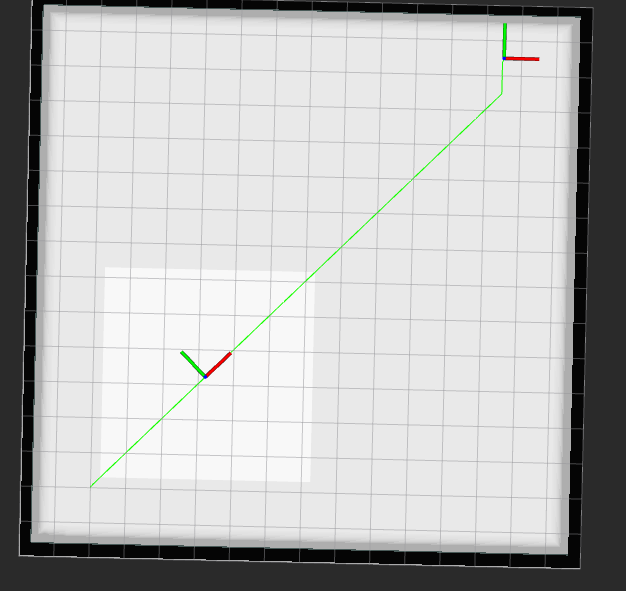
\includegraphics[width=0.9\columnwidth]{../images/manhattan_blank.png}
    \caption{Blank Map: Manhattan heuristic.}
    \label{fig:manhattan_blank}
\end{figure}
\clearpage

\subsubsection*{Euclidean}
\begin{figure}[!ht]
    \centering
    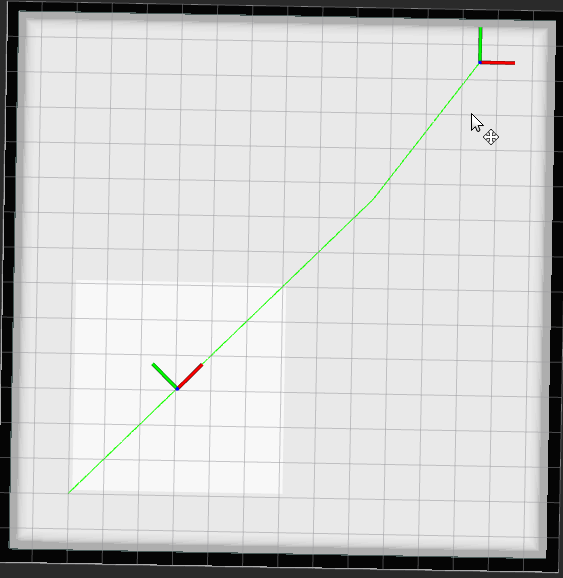
\includegraphics[width=0.9\columnwidth]{../images/euclidean_blank.png}
    \caption{Blank map: Euclidean heuristic.}
    \label{fig:euclidean_blank}
\end{figure}
\clearpage

\subsubsection*{Chebyshev}
\begin{figure}[!ht]
    \centering
    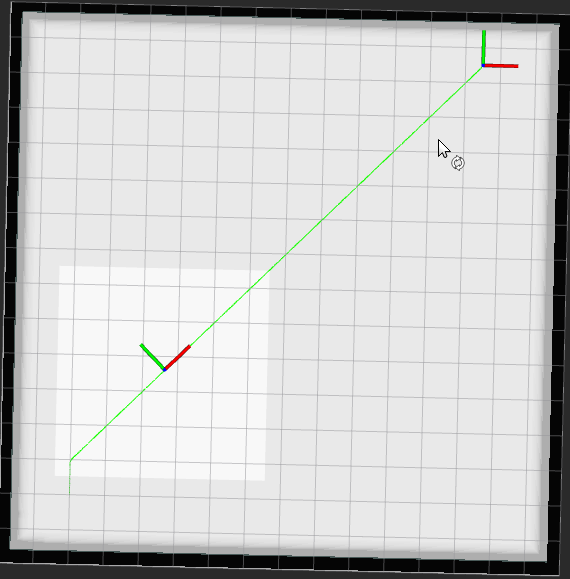
\includegraphics[width=0.9\columnwidth]{../images/chebyshev_blank.png}
    \caption{Blank map: Chebyshev heuristic.}
    \label{fig:chebyshev_blank}
\end{figure}

\clearpage


\subsection*{Corridor Map}

\subsubsection*{Manhattan}
\begin{figure}[!ht]
    \centering
    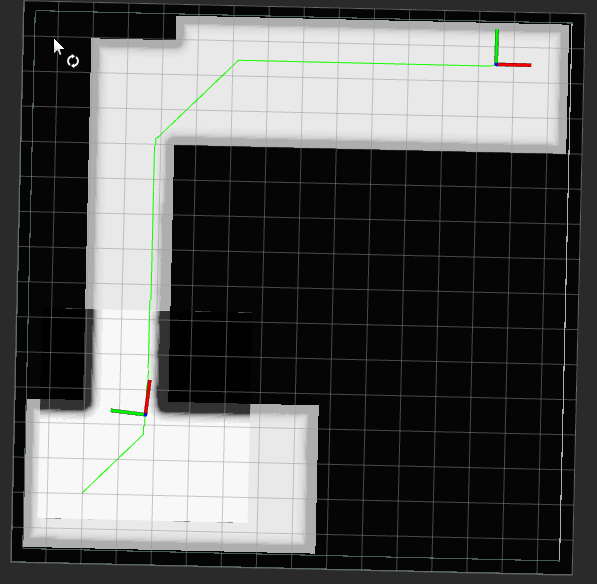
\includegraphics[width=0.9\columnwidth]{../images/manhattan_corridor.png}
    \caption{Corridor map: Manhattan heuristic.}
    \label{fig:manhattan_open}
\end{figure}
\clearpage

\subsubsection*{Euclidean}
\begin{figure}[!ht]
    \centering
    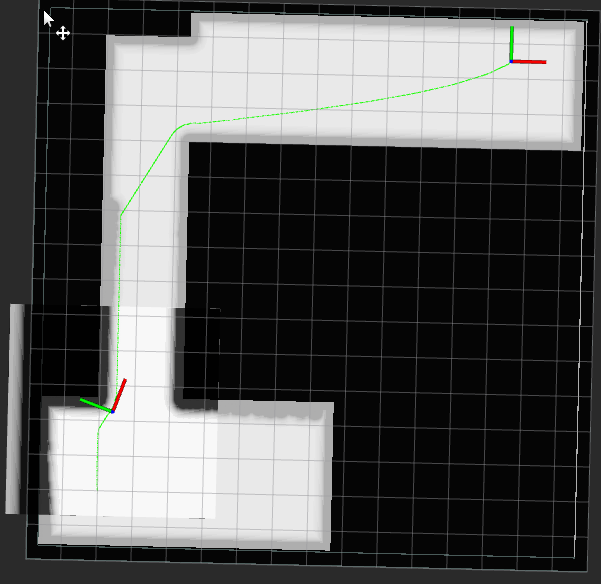
\includegraphics[width=0.9\columnwidth]{../images/euclidean_corridor.png}
    \caption{Corridor map: Euclidean heuristic.}
    \label{fig:euclidean_open}
\end{figure}
\clearpage

\subsubsection*{Chebyshev}
\begin{figure}[!ht]
    \centering
    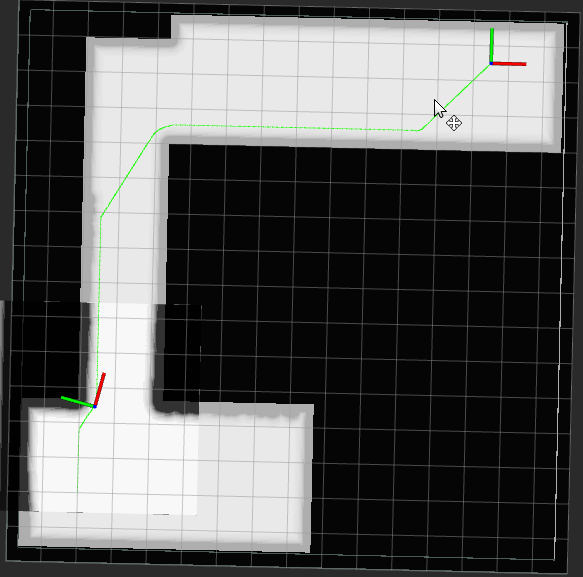
\includegraphics[width=0.9\columnwidth]{../images/chebyshev_corridor.png}
    \caption{Open space map: Chebyshev heuristic.}
    \label{fig:chebyshev_open}
\end{figure}

\clearpage
\end{document}